\lstset{language=VBScript,
        basicstyle=\footnotesize\ttfamily,
        breaklines=true,
        tabsize=2,
        numbers=left,
        numberstyle=\tiny,
        numbersep=7pt,
        showspaces=false,
        keywordstyle=\color{Blue}\textbf,
        commentstyle=\color{Red}\emph,
        showstringspaces=false,
        stringstyle=\color{BurntOrange}
        }
\section{Instrukcja użytkownika}
%\subsection{Specyfikacja zewnętrzna}

\subsection{Ogólny opis programu}

\noindent Po uruchomieniu aplikacji pierwszym widocznym oknem, będzie ekran powitalny (Rys.~\ref{splash_screen}). U~jego dołu wyświetlony jest przebieg kontroli systemu wykonywanej każdorazowo przy~próbie włączenia programu. Podczas testu sprawdzane są:
\begin{enumerate}
\item istnienie poprawnej bazy danych i~możliwość połączenia,
\item istnienie portów szeregowych,
\item dostęp do wszystkich potrzebnych sterowników.
\end{enumerate}
\noindent W~razie potrzeby automatycznie uzupełniane~są słowniki konieczne dla poprawnego działania aplikacji.

\begin{figure}[!htb]
\centering 		
  \subfloat[Windows]{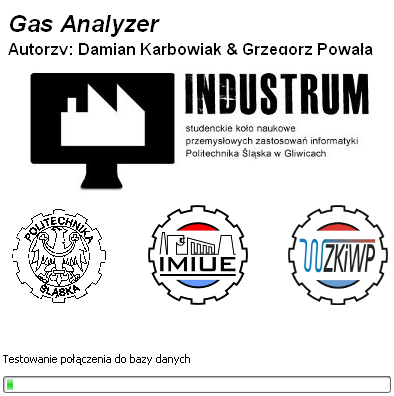
\includegraphics[width=0.45\textwidth]{images/splashScreenW}}   
  \hspace{2mm}          
  \subfloat[Linux]{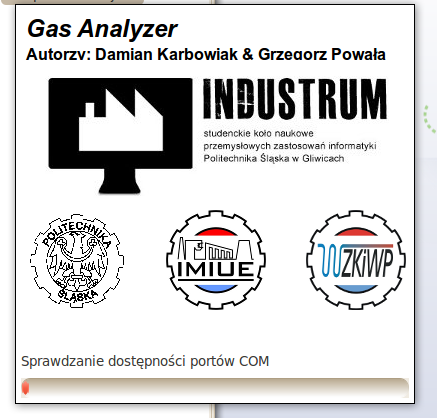
\includegraphics[width=0.45\textwidth]{images/splashScreenL}}
\caption{Okno ładowania} 	
\label{splash_screen}
\end{figure}

\noindent W~przypadku wykrycia braku elementów niezbędnych do poprawnego działania programu wyświetlony zostanie odpowiedni komunikat (Rys.~\ref{dbError} i Rys.~\ref{rxtxError}).

\begin{figure}[!htb]
\centering 		
  \subfloat[Windows]{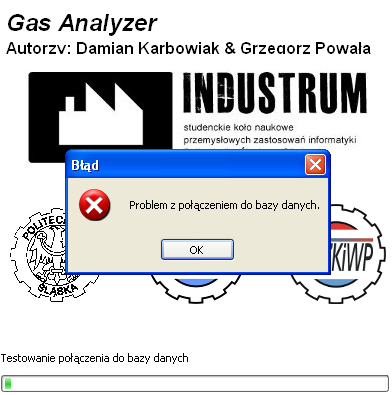
\includegraphics[width=0.35\textwidth]{images/dbErrorW}}    
  \hspace{2mm}
  \subfloat[Linux]{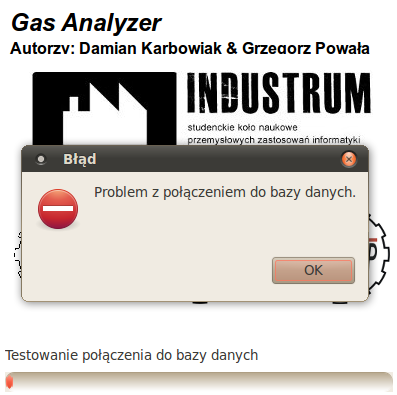
\includegraphics[width=0.35\textwidth]{images/dbErrorL}}
\caption{Komunikat o błędzie łączenia do bazy danych} 	
\label{dbError}
\end{figure}

\begin{figure}[!htb]
\centering 		
  \subfloat[Windows]{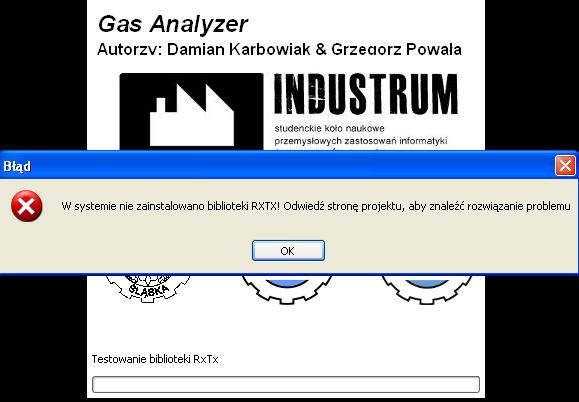
\includegraphics[width=0.45\textwidth]{images/rxtxErrorW}}    
  \hspace{2mm}
  \subfloat[Linux]{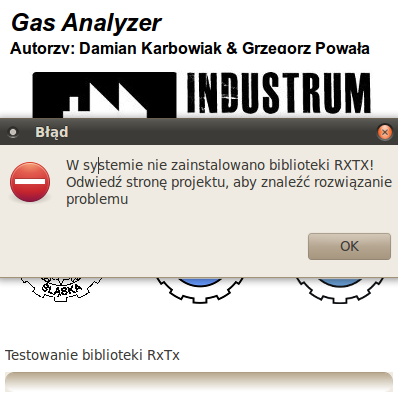
\includegraphics[width=0.45\textwidth]{images/rxtxErrorL}}
\caption{Okno błędu braku biblioteki RXTX} 	
\label{rxtxError}
\end{figure}

\noindent Po wykonaniu wszystkich testów i~sprawdzeniu poprawności konfiguracji systemu użytkownik zostaje przeniesiony do głównego okna aplikacji (Rys.~\ref{main}). Bezpośrednio po uruchomieniu większość funkcji jest nieaktywna. W~celu ich uaktywnienia konieczne jest utworzenie bądź wczytanie istniejącego pomiaru. Operacje te są opisane w~dalszej części instrukcji. W~tym momencie można zaobserwować budowę programu. Na~górze okna widoczne są menu.
\begin{itemize}
\item Menu ,,Plik'': umożliwia wykonanie podstawowych akcji niezbędnych podczas codziennego użytkowania programu tj.~utworzenie i~otworzenie pomiaru oraz wyłączenie programu. Dostępne są następujące funkcjonalności:
\begin{itemize}
\item ,,Nowy pomiar'': umożliwia utworzenie nowego pomiaru (Rys.~\ref{newSurveyFilled}),

\begin{figure}[!htb]
\centering 		
  \subfloat[Windows]{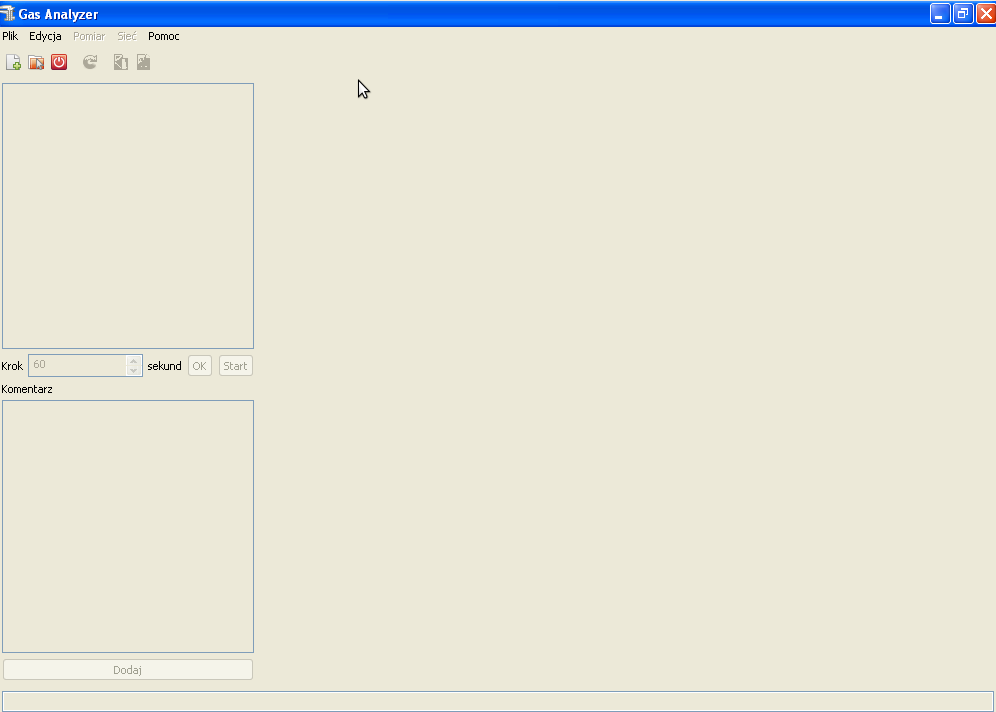
\includegraphics[width=0.49\textwidth]{images/mainW}}    
  \hspace{1mm}
  \subfloat[Linux]{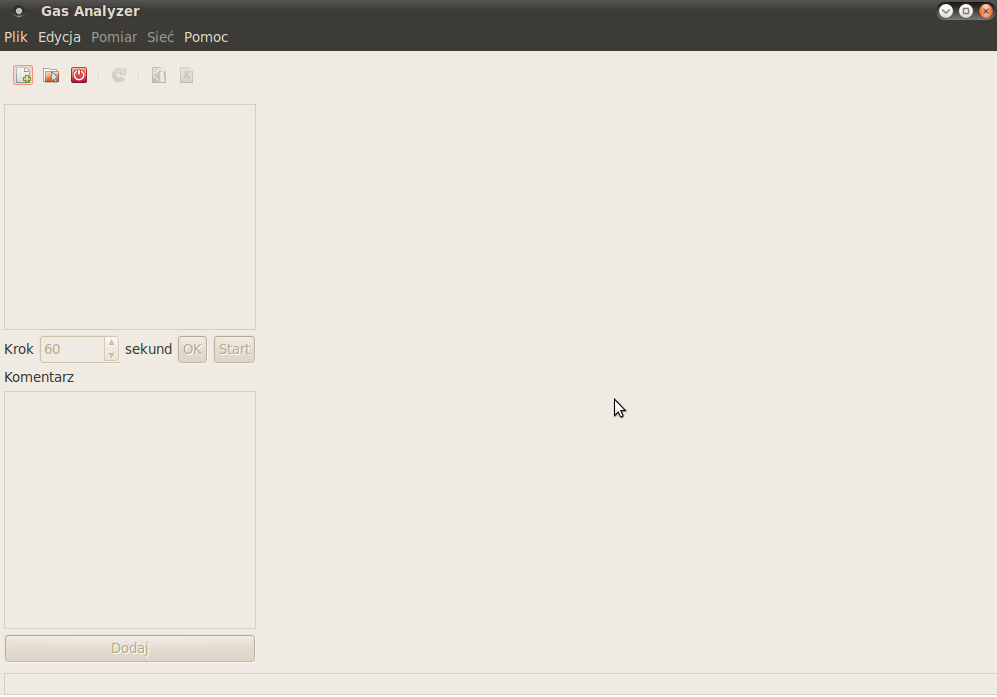
\includegraphics[width=0.49\textwidth]{images/mainL}}
\caption{Okno główne programu} 	
\label{main}
\end{figure}

\begin{figure}[!htb]
\centering 		
  \subfloat[Windows]{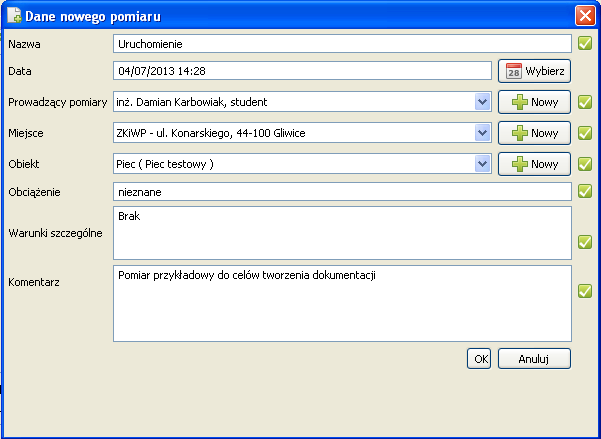
\includegraphics[width=0.45\textwidth]{images/newSurveyFilledW}}    
  \hspace{2mm}
  \subfloat[Linux]{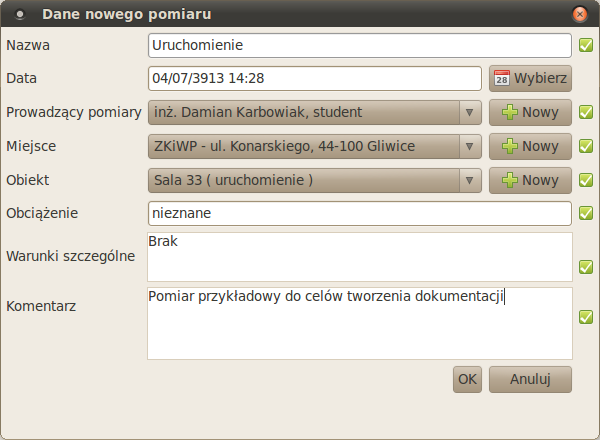
\includegraphics[width=0.45\textwidth]{images/newSurveyFilledL}}
\caption{Okno dodawania pomiaru po prawidłowym wypełnieniu} 	
\label{newSurveyFilled}
\end{figure}

\item ,,Otwórz pomiar'': umożliwia otworzenie i~kontynuowanie poprzednio utworzonego pomiaru (Rys.~\ref{openSurvey}),

\begin{figure}[!htb]
\centering 		
  \subfloat[Windows]{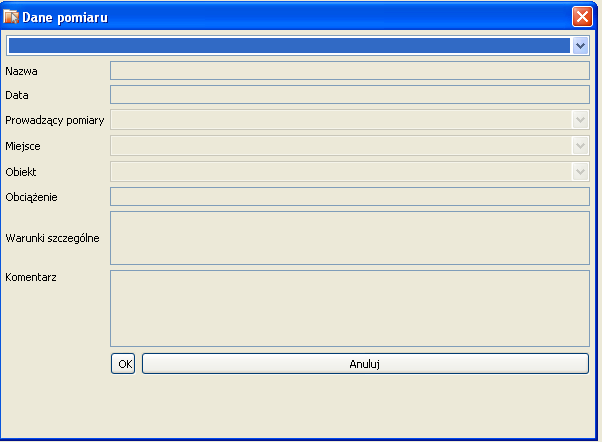
\includegraphics[width=0.45\textwidth]{images/openSurveyW}}    
  \hspace{2mm}
  \subfloat[Linux]{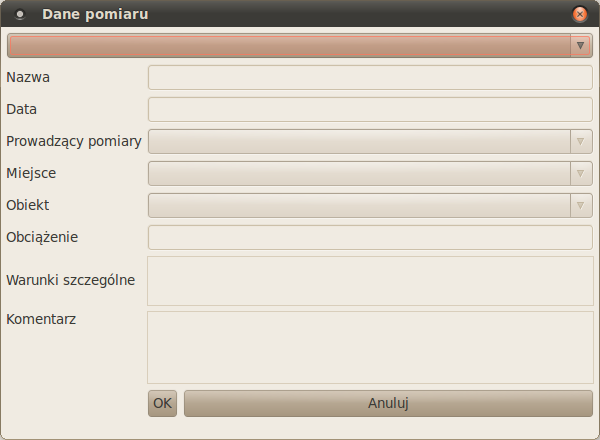
\includegraphics[width=0.45\textwidth]{images/openSurveyL}}
\caption{Okno otwierania pomiaru} 	
\label{openSurvey}
\end{figure}

\item ,,Wyjście'': pozwala na opuszczenie aplikacji.
\end{itemize}

\item Menu ,,Edycja'': umożliwia edycję wszelkich parametrów pomiaru. Zaliczają się do nich:
\begin{itemize}
\item ,,Edytuj prowadzących pomiar'': umożliwia edycję danych o~osobach przeprowadzających pomiar. Prócz danych personalnych przechowywane są informacje o tytule naukowym i~pełnionej funkcji (Rys.~\ref{editUser}),

\begin{figure}[!htb]
\centering 		
  \subfloat[Windows]{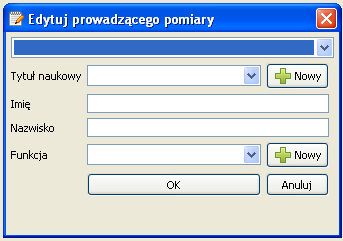
\includegraphics[width=0.45\textwidth]{images/editUserW}}    
  \hspace{2mm}
  \subfloat[Linux]{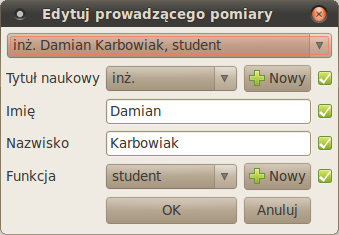
\includegraphics[width=0.45\textwidth]{images/editUserL}}
\caption{Okno edycji danych użytkownika} 	
\label{editUser}
\end{figure}

\item ,,Edytuj tytuły'': umożliwia edycję tytułów naukowych (Rys.~\ref{editTitle}),

\begin{figure}[!htb]
\centering 		
  \subfloat[Windows]{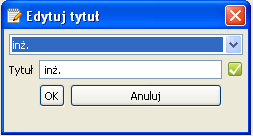
\includegraphics[width=0.45\textwidth]{images/editTitleW}}    
  \hspace{2mm}
  \subfloat[Linux]{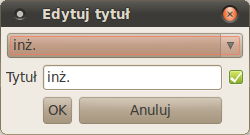
\includegraphics[width=0.45\textwidth]{images/editTitleL}}
\caption{Okno edycji tytułów naukowych} 	
\label{editTitle}
\end{figure}

\item ,,Edytuj funkcje'': umożliwia edycję funkcji, które są przypisane użytkownikom pomiaru np. ,,prowadzący pomiar'', ,,obserwator'', ,,kontroler'', ,,student'' (Rys.~\ref{editFunction}),

\begin{figure}[!htb]
\centering 		
  \subfloat[Windows]{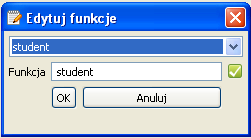
\includegraphics[width=0.45\textwidth]{images/editfFunctionW}}    
  \hspace{2mm}
  \subfloat[Linux]{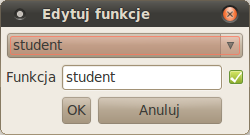
\includegraphics[width=0.45\textwidth]{images/editfFunctionL}}
\caption{Okno edycji funkcji} 	
\label{editFunction}
\end{figure}

\item ,,Edytuj miejsca'': umożliwia edycję informacji o miejscu, w którym odbywa się pomiar (Rys.~\ref{editPlace}),

\begin{figure}[!htb]
\centering 		
  \subfloat[Windows]{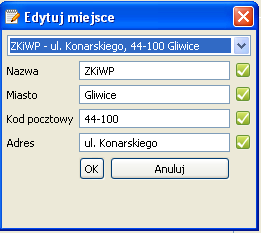
\includegraphics[width=0.45\textwidth]{images/editPlaceW}}    
  \hspace{2mm}
  \subfloat[Linux]{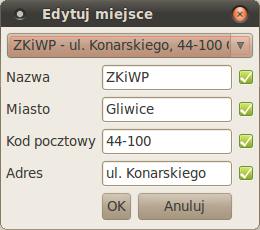
\includegraphics[width=0.45\textwidth]{images/editPlaceL}}
\caption{Okno edycji miejsc} 	
\label{editPlace}
\end{figure}

\item ,,Edytuj obiekty'': umożliwia edycję obiektów będących przedmiotem pomiaru (Rys.~\ref{editObject}).

\begin{figure}[!htb]
\centering 		
  \subfloat[Windows]{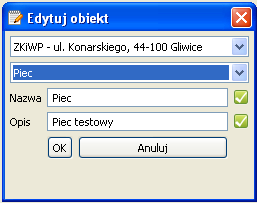
\includegraphics[width=0.45\textwidth]{images/editObjectW}}    
  \hspace{2mm}
  \subfloat[Linux]{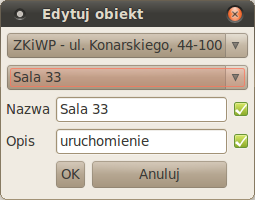
\includegraphics[width=0.45\textwidth]{images/editObjectL}}
\caption{Okno edycji obiektów} 	
\label{editObject}
\end{figure}

\end{itemize}
\item Menu ,,Pomiar'': staje się aktywne po utworzeniu lub otworzeniu pomiaru i~nawiązaniu połączenia z~wybranym koncentratorem. Umożliwia konfigurację parametrów aktualnie prowadzonego pomiaru. Daje on następujące możliwości:
\begin{itemize}
\item ,,Edytuj urządzenia'': umożliwia edycję parametrów urządzeń podłączonych do sieci tj. nazwa i~typ urządzenia oraz precyzja pomiaru poszczególnych składników (Rys.~\ref{editDevice}).

\begin{figure}[!htb]
\centering 		
  \subfloat[Windows]{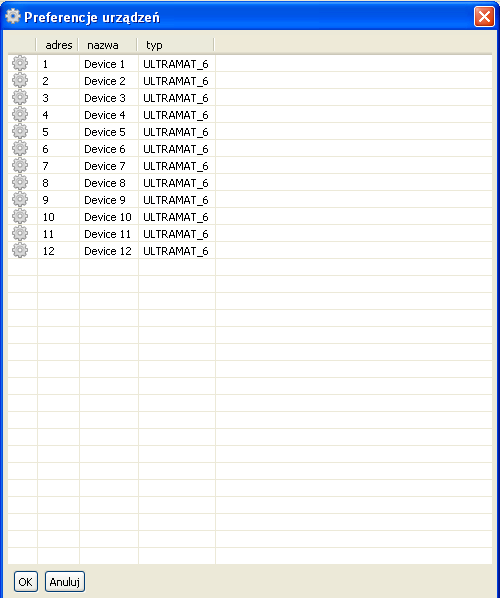
\includegraphics[width=0.4\textwidth]{images/editDeviceW}}    
  \hspace{2mm}
  \subfloat[Linux]{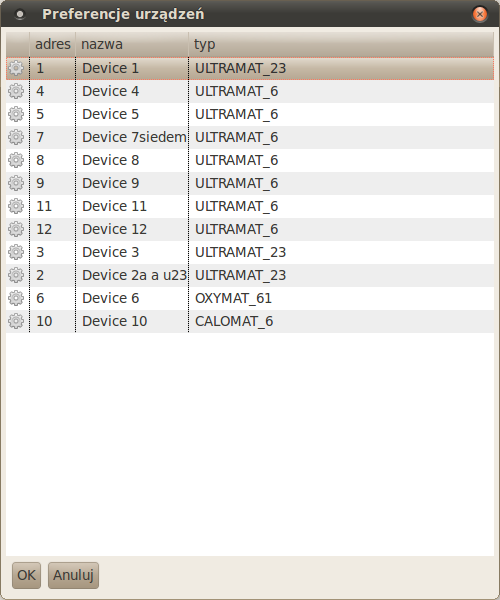
\includegraphics[width=0.4\textwidth]{images/editDeviceL}}
\caption{Okno edycji danych urządzeń} 	
\label{editDevice}
\end{figure}

Po kliknięciu na ikonę 
\includegraphics[scale=0.75]{images/preferences} dostępne są opcje umożliwiające zmianę precyzji pomiaru poszczególnych składników oraz wybranie składników, których pomiar umożliwia urządzenie (Rys.~\ref{editPrecision}).

\begin{figure}[!htb]
\centering 		
  \subfloat[Windows]{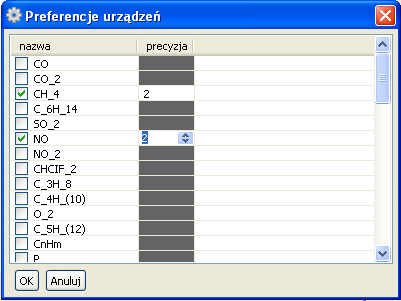
\includegraphics[width=0.45\textwidth]{images/editPrecisionW}}    
  \hspace{2mm}
  \subfloat[Linux]{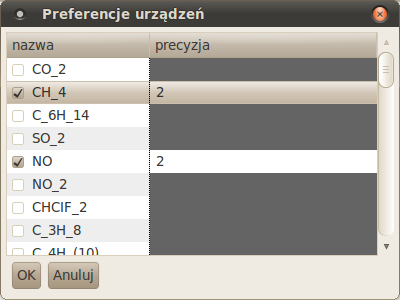
\includegraphics[width=0.45\textwidth]{images/editPrecisionL}}
\caption{Okno edycji precyzji pomiarowej} 	
\label{editPrecision}
\end{figure}

\begin{tikzpicture}
\node[color=black!80,draw=red!80,fill=red!30,shape=rectangle,rounded corners=0.5ex,
text width=36em, text centered] at (4,0) 
{
\textbf{UWAGA}\linebreak
Podczas edycji parametrów urządzeń pomiarowych dostępnych jest zawsze 12 urządzeń. Jest to maksymalna liczba urządzeń, których jednoczesną pracę przewiduje protokół ELAN. Podczas realizacji pomiaru podłączona może być mniejsza liczba urządzeń, ale możliwa jest edycja parametrów wszystkich. W celu sprawdzenia, które urządzenie konfigurujemy należy posłużyć się niezmiennym po stronie aplikacji adresem urządzenia. Adres ten jest konfigurowalny z poziomu panelu sterowania tego urządzenia.
};
\end{tikzpicture}

\item ,,Preferencje'': umożliwia edycję informacji o aktualnie trwającym pomiarze (Rys.~\ref{editSurvey}).

\begin{figure}[!htb]
\centering 		
  \subfloat[Windows]{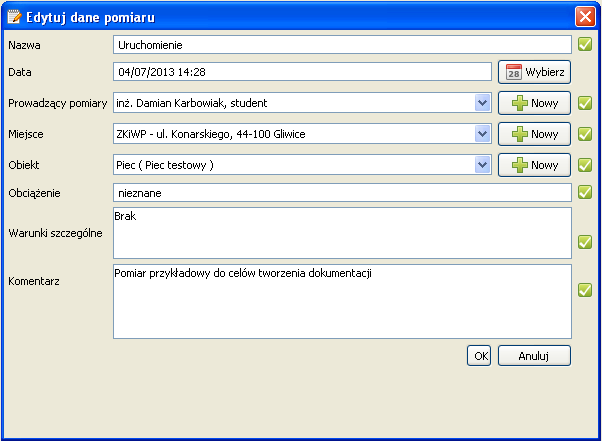
\includegraphics[width=0.45\textwidth]{images/editSurveyW}}    
  \hspace{2mm}
  \subfloat[Linux]{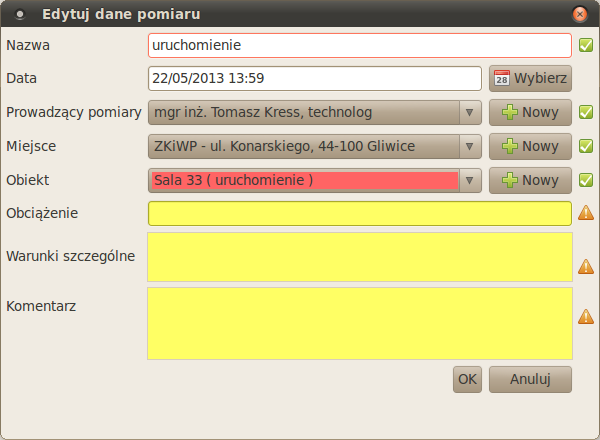
\includegraphics[width=0.45\textwidth]{images/editSurveyL}}
\caption{Okno edycji preferencji aktualnego pomiaru} 	
\label{editSurvey}
\end{figure}

\end{itemize}
\item Menu ,,Sieć'': jest to obecnie najuboższe menu, zawiera tylko jedną funkcjonalność:
\begin{itemize}
\item ,,Odśwież'': umożliwia odświeżenie listy dostępnych portów.
\end{itemize}
\item Menu ,,Pomoc'': pozwala na zgłoszenie błędów oraz sugestii twórcom programu, funkcje te korzystają ze standardowego klienta pocztowego dostępnego w systemie, odpowiadają za:
\begin{itemize}
\item ,,Zgłoś błąd'': umożliwia zgłoszenie krytycznego błędu twórcom oprogramowania, którzy poczynią wszelkie starania aby usunąć usterkę,
\item ,,Zgłoś sugestię'': umożliwia zasugerowanie funkcjonalności lub poprawę istniejącej, nie należy zgłaszać za jej pomocą krytycznych błędów uniemożliwiających pracę z~oprogramowaniem,
\item ,,O programie'': wyświetla okno z krótką informacją o~użytkowanym programie.
\end{itemize}
\textit{Uprasza się użytkowników o~rozsądne korzystanie z~funkcji kontaktu z~twórcami oprogramowania oraz precyzyjne wyrażanie myśli.}
\end{itemize}

\begin{tikzpicture}
\node[color=black!80,draw=red!80,fill=red!30,shape=rectangle,rounded corners=0.5ex,
text width=36em, text centered] at (4,0) 
{
\textbf{UWAGA}\linebreak
W~celu wykonania pomiaru konieczne jest uzupełnienie informacji o~minimum jednym użytkowniku oraz o~przynajmniej jednym obiekcie będącym przedmiotem pomiaru. W~ramach jednego miejsca może istnieć wiele obiektów.
};
\end{tikzpicture}
\newpage
\subsection{Krótka instrukcja wykonania pomiaru}

Oprogramowanie zostało zaprojektowane tak, aby było jak najbardziej intuicyjne i~przystępne, a~funkcjonalnością jak najbardziej zbliżone do dotychczas przeprowadzonych pomiarów. Część funkcji oprogramowania nie została zawarta w~instrukcji gdyż są one widoczne zaraz po rozpoczęciu pomiaru, a~użytkownik nie ma możliwości ich konfiguracji. Tak jest między innymi z~oknem błędów i~ostrzeżeń widocznym na dole okna programu, oraz z~wszelkimi polami wyświetlającymi aktualny wynik pomiarów. \\
\\
W tym krótkim rozdziale przedstawiona zostanie krótka instrukcja, która krok po kroku przeprowadzi użytkownika przez kolejne etapy tworzenia, uruchamiania i raportowania pomiarów. 
\begin{enumerate}
\item Uruchom program i~zaczekaj aż konfiguracja środowiska pomyślnie się zakończy.
\item Utwórz nowy pomiar. W tym celu kliknij \textit{Plik $\rightarrow$ Nowy pomiar} i~uzupełnij wszystkie wymagane pola.
\item Na liście znajdź tą do której podpięte są analizatory. Najprawdopodobniej będzie tam dostępna tylko jedna sieć. Może też nie być żadnej. W~takim wypadku kliknij \textit{Sieć $\rightarrow$ Odśwież} w~celu wykrycia dostępnych urządzeń.
\item Kiedy właściwa sieć została wykryta kliknij na nią prawym przyciskiem myszy i~wybierz opcję \textit{Połącz} (Rys.~\ref{connect}). Po nawiązaniu połączenia można już oglądać aktualne wyniki pomiarów (Rys.~\ref{detailNetwork}). Pomiary są prezentowane dopiero, kiedy urządzenie jest w~pełni gotowe do pracy. Jeśli występują jakiekolwiek problemy jest wyświetlana stosowna informacja.
\begin{figure}[!htb]
\centering 		
  \subfloat[Windows]{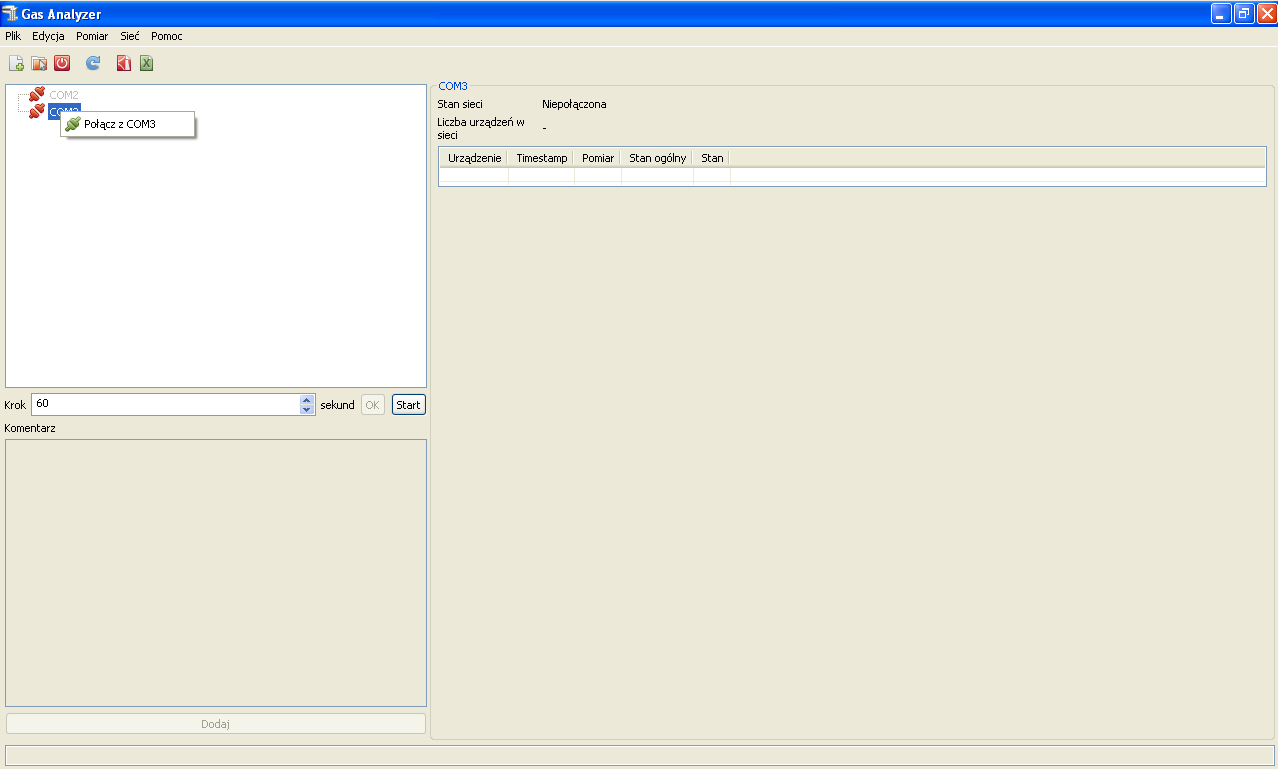
\includegraphics[width=0.49\textwidth]{images/connectW}}    
  \hspace{1mm}
  \subfloat[Linux]{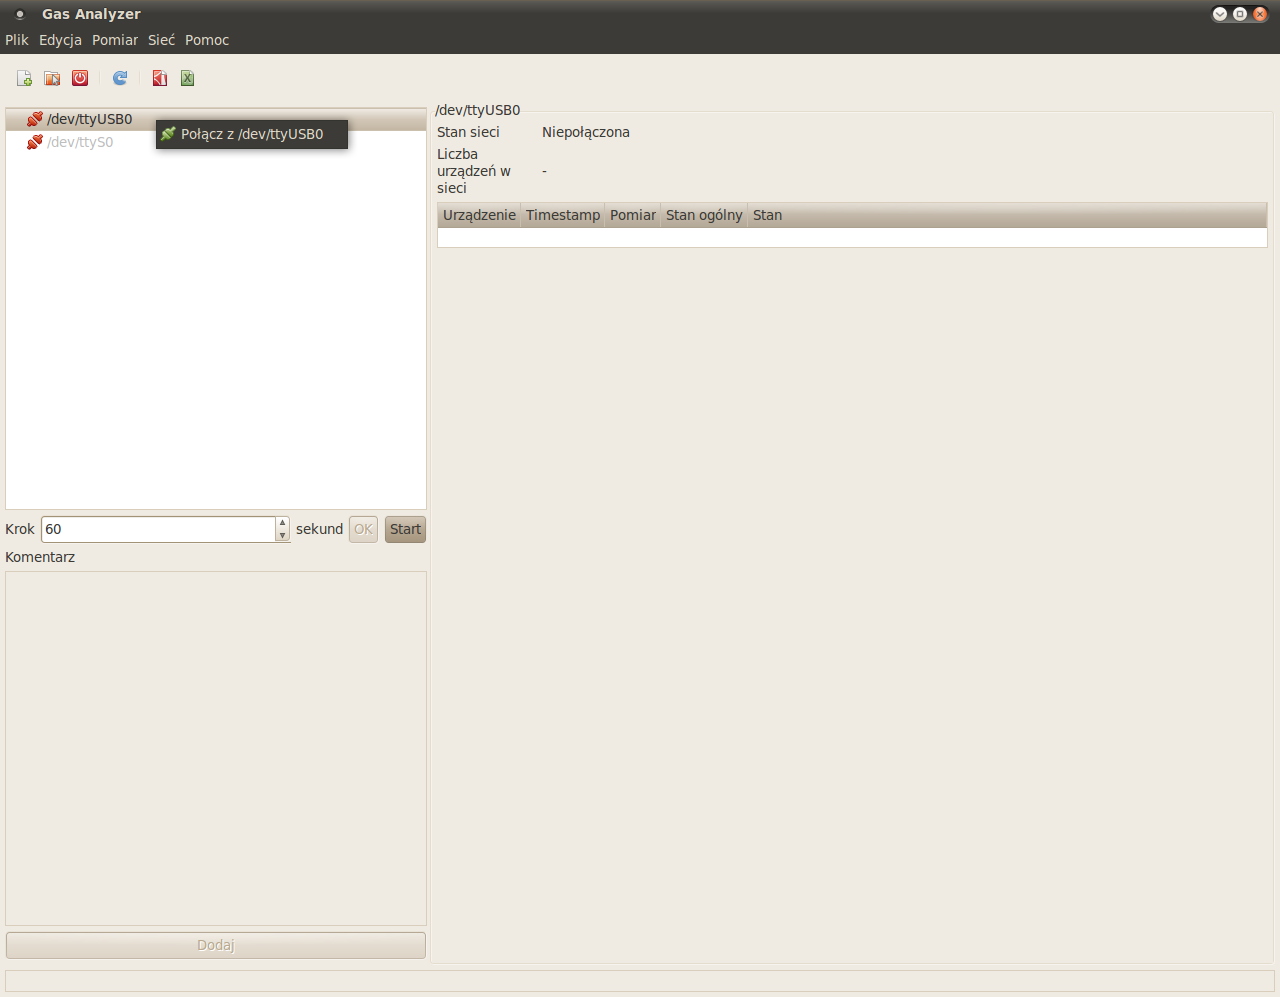
\includegraphics[width=0.49\textwidth]{images/connectL}}
\caption{Łączenie z siecią} 	
\label{connect}
\end{figure}
\begin{figure}[!htb]
\centering 		
  \subfloat[Windows]{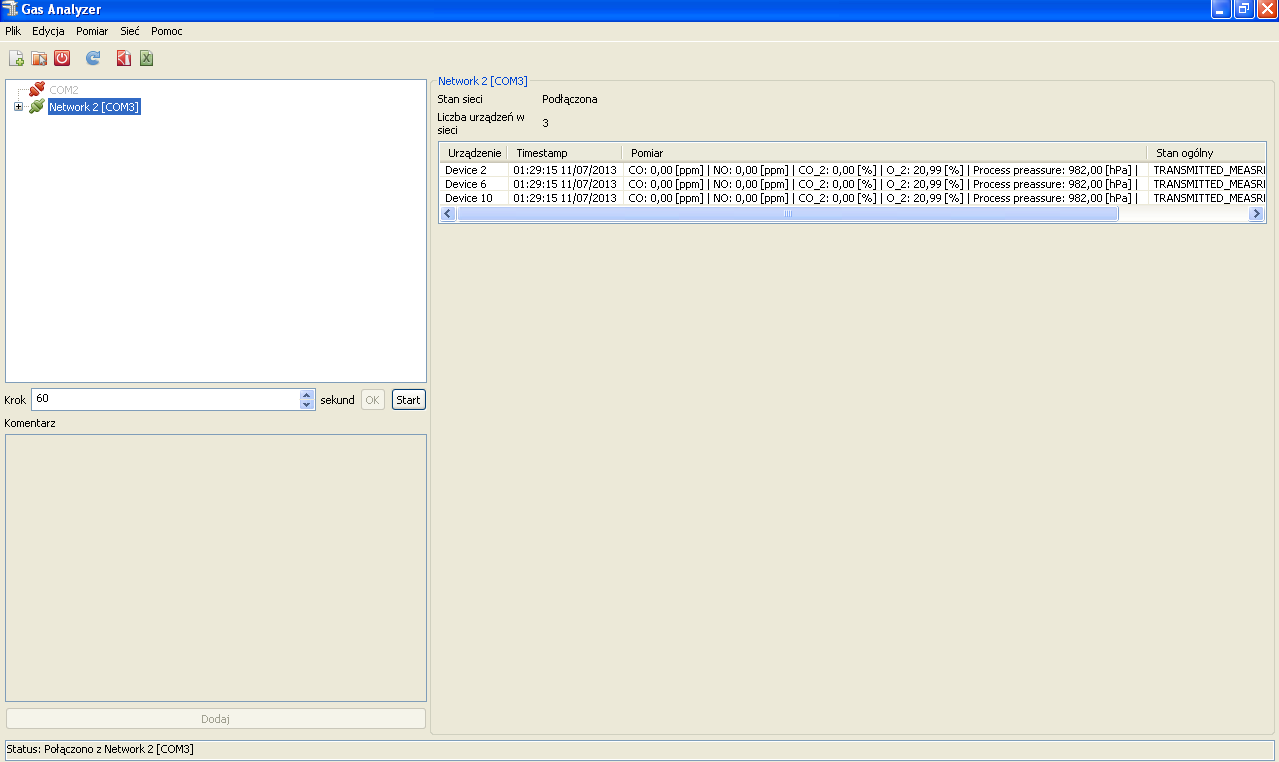
\includegraphics[width=0.49\textwidth]{images/detailNetworkW}}    
  \hspace{1mm}
  \subfloat[Linux]{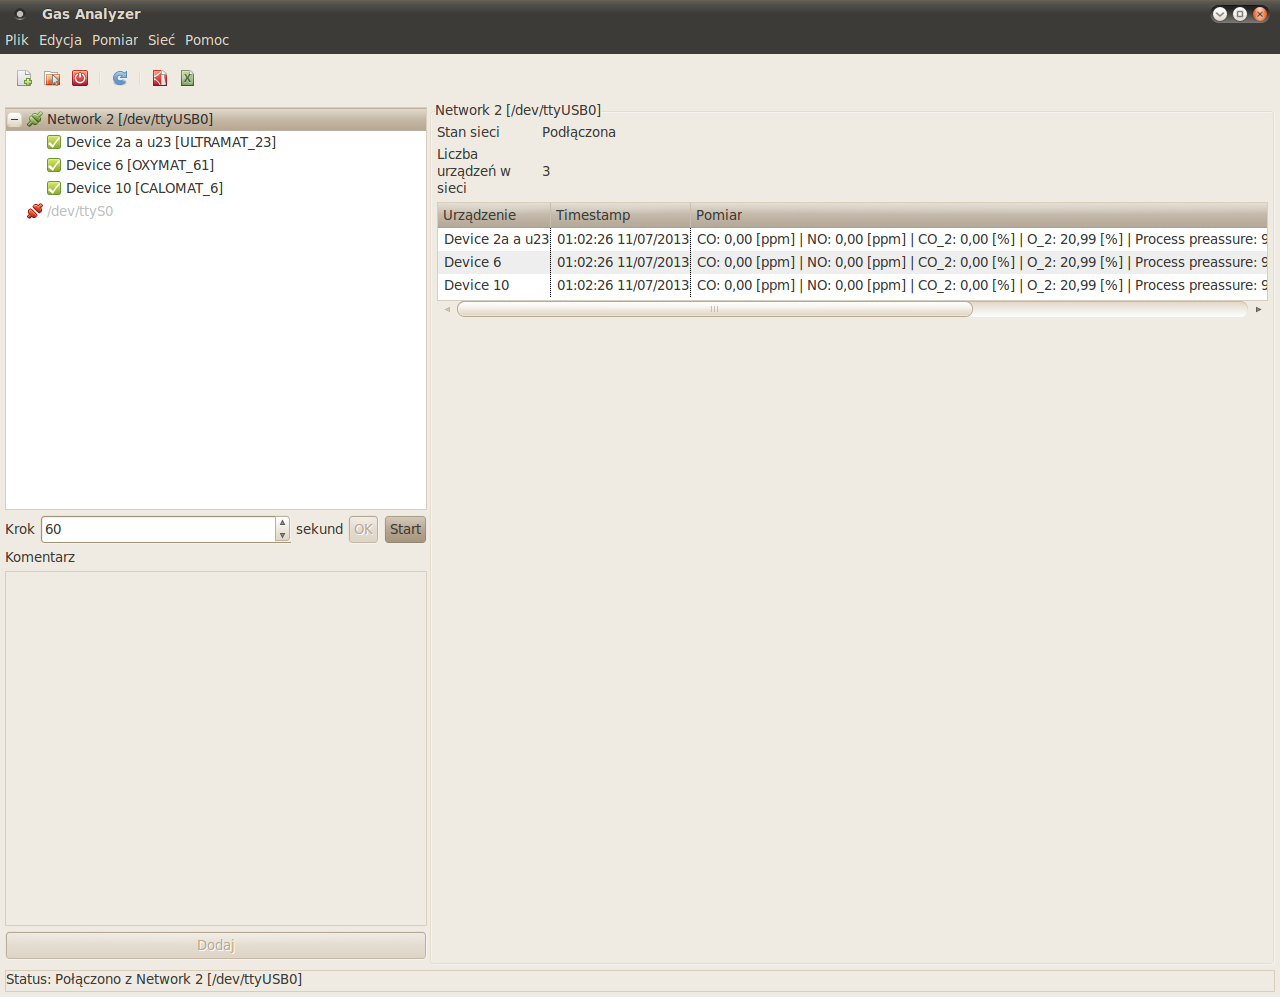
\includegraphics[width=0.49\textwidth]{images/detailNetworkL}}
\caption{Szczegółowy widok sieci} 	
\label{detailNetwork}
\end{figure}
\item W~celu rozpoczęcia zapisu danych do bazy danych kliknij przycisk \textit{Start}. Dane są zapisywane z~predefiniowanym krokiem 60[s]. Oznacza to, że co 60[s] aktualny pomiar ze wszystkich urządzeń zostanie zapisany. W celu zmiany interwału pomiarowego należy wybrać żądaną wartość kroku w~polu \textit{Krok} i~kliknąć \textit{OK}.
\item W każdej chwili do pomiaru można dodać dowolny komentarz. W~tym celu uzupełnij pole \textit{Komentarz} i~kliknij \textit{Dodaj}. Komentarz zostanie dodany do następnego pomiaru zapisanego w~bazie. 
\item Pomiar zatrzymuje się po naciśnięciu przycisku \textit{Stop}.
\item Po zatrzymaniu pomiaru możliwe jest wygenerowanie plików raportu zarówno w~postaci pliku pdf (ikona 
\includegraphics[scale=0.75]{images/pdfIco})(Rys.~\ref{reportPDFfinal}) jak i~arkusza kalkulacyjnego (ikona 
\includegraphics[scale=0.75]{images/excel})(Rys.~\ref{reportXLSfinal}).
\end{enumerate}

\begin{figure}[!htb] 	\centering 	
\includegraphics[width=0.9\textwidth]{images/pdf} 	\caption{Przykładowy raport PDF} \label{reportPDFfinal} \end{figure} 

\begin{figure}[!htb] 	\centering 	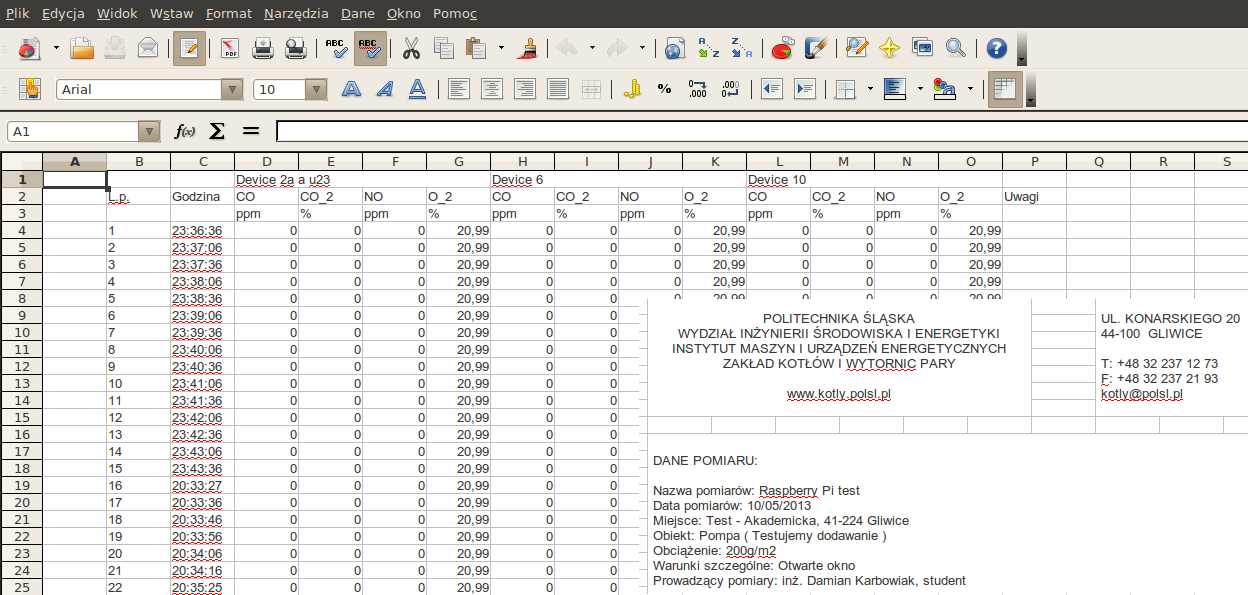
\includegraphics[width=0.99\textwidth]{images/xls} 	\caption{Przykładowy raport XLS} \label{reportXLSfinal} \end{figure} 

Na zakończenie tej krótkiej instrukcji warto udzielić kilku rad, które mogą przydać się w~codziennej eksploatacji oprogramowania.
\begin{itemize}
\item Pomiar można utworzyć wcześniej uzupełniając wszelkie potrzebne dane, a~na stanowisku pomiarowym jedynie otworzyć przygotowany wcześniej pomiar. Korzystając z~tej samej funkcjonalności można w dowolnej chwili kontynuować niegdyś zakończony pomiar.
\item Pliki raportów można generować w~dowolnej chwili. Wystarczy otworzyć przeprowadzony pomiar. Urządzenia nie muszą być wtedy podłączone, jak również nie musi zostać wykryta sieć.
\end{itemize}

\subsection{Instalacja i pierwsze uruchomienie}
Aby rozpocząć użytkowanie programu należy zainstalować:
\begin{enumerate}
\item Jave w wersji 6 lub 7,
\item PostgreSQL najlepiej w wersji 8.4,
\item Bibliotekę RXTX zgodnie z opisem twórcy.
\end{enumerate}

Następnie należy uruchomić program pgAdmin III i wywołać w nim dwa skrypty SQL: \textit{GasAnalyzer.sql} oraz \textit{0\_0\_1\_to\_0.0.2.sql}.
Dzięki temu zostanie dodany odpowiedni użytkownik, baza danych oraz tabele.
\\
\\
Na koniec wystarczy skopiować w dowolne miejsce plik wykonywalny JAR zgodny z wersją wirtualnej maszyny Javy i uruchomić go.